% !TEX program = lualatex
% Document Class
\documentclass[12pt]{article}

% Packages
\usepackage{amsmath, amsthm, amssymb, mathtools} % Math tools
\usepackage{enumitem} % Customizable lists
\usepackage{geometry} % Better page layout
\usepackage{fancyhdr} % Headers and footers
\usepackage{hyperref} % Clickable links
\usepackage{tikz} % For diagrams (optional)
\usepackage{bookmark}
\usepackage{fontspec}
\usepackage{titlesec}
\usepackage{mathptmx}

\setmainfont{TeX Gyre Pagella}

\titleformat{\title}[display]
		{\normalfont\bfseries\centering}
		{\vspace{2cm}\thetitle}
		{0.5cm}
		{\Huge}
\titleformat{\author}[display]
    {\normalfont\centering}
    {\vspace{1.5cm}\theauthor}
    {0.5cm}
    {\Large}
\titleformat{\date}[display]
    {\normalfont\centering}
    {\vspace{1.5cm}\thedate}
    {0.5cm}
    {\Large}

% Page Setup
\geometry{a4paper, margin=1in}
\pagestyle{fancy}
\fancyhf{}
\fancyhead[R]{DiskMat - Kordamisülesanded}
\fancyhead[L]{\nouppercase{\leftmark}}
\fancyfoot[C]{\thepage}

% Theorem Environments
\newtheorem{theorem}{Teoreem}[section]
\newtheorem{lemma}[theorem]{Lemma}
\newtheorem{corollary}[theorem]{Corollary}
\newtheorem{proposition}[theorem]{Proposition}
\newtheorem{definition}[theorem]{Definitsioon}
\newtheorem{example}[theorem]{Näide}
\newtheorem{remark}[theorem]{Remark}

% Custom Problem Environment
\newenvironment{problem}[1][]{
    \begin{enumerate}[label=\textbf{Harjutus \arabic*.}, ref=#1, leftmargin=*, topsep=0.5em]
}{\end{enumerate}}

% Custom Solution Environment
\newenvironment{solution}{
    \begin{proof}[Solution]
}{\end{proof}}

% Shortcuts for Common Notations
\newcommand{\Z}{\mathbb{Z}} % Integers
\newcommand{\N}{\mathbb{N}} % Natural numbers
\newcommand{\R}{\mathbb{R}} % Real numbers
\newcommand{\Q}{\mathbb{Q}} % Rational numbers
\newcommand{\C}{\mathbb{C}} % Complex numbers
\newcommand{\set}[1]{\{#1\}} % Set notation
\newcommand{\abs}[1]{\lvert #1 \rvert} % Absolute value
\newcommand{\floor}[1]{\lfloor #1 \rfloor} % Floor function
\newcommand{\ceil}[1]{\lceil #1 \rceil} % Ceiling function

% Document Begins
\begin{document}

% Title
\title{Diskreetse Matemaatika Kordamisülesanded} 
\author{Karl Marten Jaaska}
\maketitle

\newpage 
% Table of Contents
\tableofcontents
\newpage

% Sections
\section{Kvantorid}
\begin{theorem}[Definitsioon]
\leavevmode

Kvantoreid on kahte tüüpi: üldsuse kvantor $\forall$ ja eksistentsikvantor $\exists$.
\end{theorem}
\noindent
Kvantoreid kasutatakse peamiselt selle tõttu, et väita kompaktsemal viisil, et 
predikaat kehtib mingis oma määramispiirkonnas.
\newline
\begin{example}
$\mathbf{P(x)} \equiv (x > 2) \wedge (x < 4)$ \\ 
\\ Esmalt rakendame predikaadile üldsuse kvantorit ning seejärel olemasolu kvantorit ja leiame tulemuseks olevate 
lausete tõeväärtused: \\ 
\\ $\forall\mathbf{x}\mathbf{P(x)}$ [vale] \\ 
\\ $\exists\mathbf{x}\mathbf{P(x)}$ [õige] \\
\end{example}
\begin{example}
	Olgu naturaalarvulise määramispiirkonnaga ühekohalised predikaadid: \\ 
	\\
	$\mathbf{P(x)} \equiv \mathit{\mathbf{x}}$ jagub $3$-ga \\ 
	\\
	$\mathbf{Q(x)} \equiv \mathbf{x}$ jagub $4$-ga \\ 
	\\ 
	$\mathbf{S(x)} \equiv \mathbf{x}$ jagub $12$-ga \\ 
	\\ 
	$\mathbf{T(x)} \equiv \mathbf{P(x)} \wedge \mathbf{Q(x)}$ \\ 
	\begin{solution}
	.... siis: $\mathbf{S(x)} \equiv \mathbf{T(x)}$ \\
	\end{solution}
\end{example}

\begin{example} 
	Leiame kahekohalise predikaadi $\mathbf{P(x,y)}$ tõenäosuspiirkonna: \\ 
	\\ 
	\[ 
		\mathbf{P(x,y)} \equiv x^2 - y^2 = 0
		\]
		\textit{$\mathbf{P(x,y)}$ on tõene kui: $(x = y) \vee (x = -y)$} \\
	

	\[
	\mathbf{P(x,y)} \equiv (x > 0) \rightarrow (y < 0)
	\]
	\textit{$\mathbf{P(x,y)}$ on tõene kui: $(x < 0) \vee (x > 0) \wedge (y<0)$} \\

 
	\[ 
	\mathbf{P(x,y)} \equiv (x > 0) \wedge (y < 0) 
	\]
\textit{$\mathbf{P(x,y)}$ on tõene kui: $(x > 0) \wedge (y < 0)$}
\end{example}

\newpage

\section{Hulgad}
\begin{definition}[Hulk]
	Mõistel \textit{hulk} ei ole definitsiooni - \textbf{hulk} on baasmõiste. \\ 
	Hulk koosneb \textbf{hulgaeelementidest}. \\ 
	\\ 
	Hulka esitatakse suurtähtedega $\mathbf{A}, \mathbf{B}, \mathbf{C}$ 
	\\ 
	\\ 
	Hulga elementide täielikku loetelu esitatakse loogsulgude vahel : 
	\textbf{\{a e i o ä ü õ\}} \\ (elementide vahel võivad olla ka komad) 
	\\ 
	\\ 
	Hulka võib esitada ka tema elementide osalise loeteluna, mis esitab mingit regulaarset 
	\\ äratuntavat seaduspära:
	\textbf{\{ ... -2, -1, 0, 1, 2 ... \}}
	\\ 
	\\ 
	Lisaks võib hulka esitada ka üldise avaldise kaudu, mis kehtib \textbf{kõigi} hulgaeelementide jaoks: \\
\\ $\mathbf{\{n \ | \ (n > 1899) \wedge (n < 2000)\}}$ \\ 
  \\ 
	$\mathbf{\{ x \ | \ mod \ 2 = 1 \}}$
	\\ 
	\\ 
	$\mathbf{\{ x \ | \ mod \ 2 = 0 \}}$
  \\ 
	\\ 
	Hulka kuulumise (ja mittekuulumise) ning osahulgaks olemise (ja mitteolemise) avaldised \\ 
	omandavad ka tõeväärtuse(d).
	\\ 
	\\ 
	$\overline{A}$ - hulga täiend \\ 
	$A \cup B$ - hulkade ühend ehk hulkade liitmine  \\ 
	$A \cap B$ - hulkade ühisosa ehk hulkade korrutamine \\ 
	$A \setminus B$ - hulkade \textbf{vahe} ehk hulkade lahtumine (A ilma B-ta või A on lahutatud hulk B) \\
	$A \ \Delta \ B$ - hulkade sümmeetriline vahe \\ 
	$0$ - tühi hulk $\varnothing$ \\ 
	$1$ - universaalhulk $\mathbf{{I}}$
\end{definition}

\begin{problem} 
	\item On antud hulgad $\mathbf{A} = \{ a \ b \ c \ d \ e \}$ ja $\mathbf{B} = \{ a \ b \ c \ d \ e \ f \ g \ h \}$ \\ \\ 
		Leida \ $\mathbf{A \cup B}$ \ \ \ $\mathbf{A \cap B}$ \ \ \ $\mathbf{A \backslash B}$ \ \ \ $\mathbf{B \backslash A}$ \ \ \ $\mathbf{A} \ \Delta \ \mathbf{B}$
\end{problem}
\begin{solution}
	\[
		\mathbf{A} \cup \mathbf{B} = {\{ \ a \ b \ c \ d \ e \ f \ g \ h \ \}} = \mathbf{B}
\] 
\[ 
	\mathbf{A} \cap \mathbf{B} = {\{ a \ b \ c \ d \ e \}}
\]
\[ 
	\mathbf{A} \backslash \mathbf{B} = {}
\]
\[ 
	\mathbf{B} \setminus \mathbf{A} = \{f \ g \ h \}
\]
\[ 
	\mathbf{A} \ \Delta \ \mathbf{B} = \mathbf{B} \setminus \mathbf{A}
\]
\\
\textit{Viimast saab järeldada ka \textbf{asendusseose} abil}:  
\[ 
	\mathbf{A} \ \Delta \ \mathbf{B} = (\mathbf{A} \setminus \mathbf{B}) \cup (\mathbf{B} \setminus \mathbf{A}) = \varnothing \cup (\mathbf{B} \setminus \mathbf{A}) = \mathbf{B} \setminus \mathbf{A}
\] 

\end{solution}

\[
\]
\newpage
\section{Graph Theory}
\begin{definition}[Graph]
A graph \( G = (V, E) \) consists of a set of vertices \( V \) and a set of edges \( E \).
\end{definition}

\begin{problem}
\item Draw a graph with 4 vertices and 5 edges.
\end{problem}

\begin{solution}
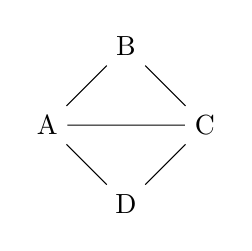
\begin{tikzpicture}
    \node (A) at (0,0) {A};
    \node (B) at (1,1) {B};
    \node (C) at (2,0) {C};
    \node (D) at (1,-1) {D};
    \draw (A) -- (B) -- (C) -- (D) -- (A) -- (C);
\end{tikzpicture}
\end{solution}

% End Document
\end{document}
